\documentclass[10pt, graphics, aspectratio=169, table]{beamer}
\usepackage{listings}
\usepackage{hyperref}
\usepackage[style=numeric]{biblatex}
\usepackage[url=true, license=full]{biblatex-license}
\usepackage{textcomp}
\usepackage{menukeys}

% -- Change to this year's color! --
\definecolor{ese}{RGB}{89, 71, 179}

\newcommand{\ra}{$\Rightarrow$\ }

\usetheme{metropolis}
\lstdefinelanguage{shell}{
	morekeywords={\$},
	keywordstyle={\color{red!50!orange}}
}
\lstset{
	basicstyle={\small\ttfamily},
	backgroundcolor={\color{green!10!white}},
	frame={trBL},
	literate={~}{$\sim$}{1},
	language={shell}
}
\setbeamercolor{frametitle}{bg=ese}
\addbibresource{ref.bib}

\title{SSH - Secure Shell}
\author{Jakob Krebs und Viktor Reusch}
\date{ESE \the\year{}}
\institute{Nerd::101 - ESE - ifsr - TU Dresden}
\titlegraphic{\hfill
\includegraphics[height=2cm]{../logo}}

\begin{document}

\maketitle

\begin{frame}<handout>{Outline}
	\tableofcontents
\end{frame}

\section{Introduction}
\begin{frame}{Motivation}
\begin{columns}
	\column{0.55\textwidth}
		\emph{Servers are versatile.}
		\begin{itemize}
			\item Uptime \ra Build a Website
			\item Location \ra Bypass Firewalls
			\item Compute Power \ra Run a Simulation
			\item Connectivity \ra Host a Game Server
		\end{itemize}
		\onslide<2->{\textbf{How do you securely control a server remotely?}}
	\column{0.45\textwidth}
		
\includegraphics[width=\textwidth]{img/servers.jpg}

		\hfill \cite{servers}
\end{columns}
\end{frame}

\begin{frame}{Overview}
	\textbf{SSH solves this problem.}
	\begin{itemize}
		\item Encrypted Network Connection
		\item Replaces insecure Telnet
		\item Remote Command-Line Interface
		\item Proxy and Port Forwarding
		\item File Transfer
	\end{itemize}
\end{frame}

\section{Basic Usage}
\begin{frame}[fragile]{Connecting to a Server}
	\begin{lstlisting}
me@my_machine:~ $ ssh remote_user@example.com
remote_user@example.com's password:
remote_user@example:~ $
	\end{lstlisting}
	\pause

	If the SSH server is not on port 22:
	\begin{lstlisting}
me@my_machine:~ $ ssh -p 1234 remote_user@example.com
	\end{lstlisting}
	\pause

	For more options:
	\begin{lstlisting}
$ man ssh
	\end{lstlisting}
\end{frame}

\begin{frame}[fragile]{Security}
	\begin{lstlisting}
me@my_machine:~ $ ssh remote_user@example.com
The authenticity of host 'example.com' can't be established.
ED25519 key fingerprint is SHA256:R[...]3.
Are you sure you want to continue connecting (yes/no)?
	\end{lstlisting}
	\pause

	\emph{Asymmetric cryptography with public and private server keys.}
	\pause

	Check fingerprint through a server control panel or with:
	\begin{lstlisting}
remote@example:~ $ ssh-keygen -lf /etc/ssh/ssh_host_ed25519_key.pub
256 SHA256:R[...]3 root@example (ED25519)
	\end{lstlisting}
\end{frame}

\begin{frame}[fragile]{Terminate a Connection}
	Terminate a connection regularly:
	\begin{lstlisting}
remote_user@example:~ $ exit
logout
Connection to example closed.
me@my_machine:~ $
	\end{lstlisting}

	Terminate an unresponding connection: \\
	\keys{\return} \keys{$\sim$} \keys{.}

	For more options: \\
	\keys{\return} \keys{$\sim$} \keys{?}
\end{frame}

\section{Keyfiles}
\begin{frame}[fragile, t]{Keyfiles}
	\centering
	\textbf{What are key files and why do you need them?} \\
	Your own public and private keys \ra More security \ra Less password hassle
	\vspace{1ex}
	\pause
	\begin{columns}[t]
	\column{0.6\textwidth}
		Generating your own key pair:
		\begin{lstlisting}
$ ssh-keygen -t ed25519 -C me@mypc
		\end{lstlisting}
		\begin{lstlisting}
$ ssh-keygen -b 4096 -t rsa
		\end{lstlisting}

		\begin{onlyenv}<3->
			Copy your \emph{public key} to a server: \textit{$\sim$/.ssh/authorized\_keys}
			\begin{lstlisting}
$ ssh-copy-id my@example.com
			\end{lstlisting}
			You can log in without a password now.
		\end{onlyenv}

	\column{0.4\textwidth}
		Resulting \textit{$\sim$/.ssh/id\_ed25519.pub}:
		\begin{lstlisting}
ssh-ed25519 AAAAC3NzaC1lZ
DI1NTE5AAAAIJDzhzcMdEg7Nz
wwgB0bdOP1pDSKv5fsN4l4q8Y
ysLLX viktor@nerd101
		\end{lstlisting}
	\end{columns}
\end{frame}

\section{Proxying}
\begin{frame}[fragile]{ProxyJump}
	\textbf{Connect to a not directly accessible server:}
	\begin{lstlisting}
$ ssh -J proxy.example.org:22 server.example.org
	\end{lstlisting}
	\begin{center}
		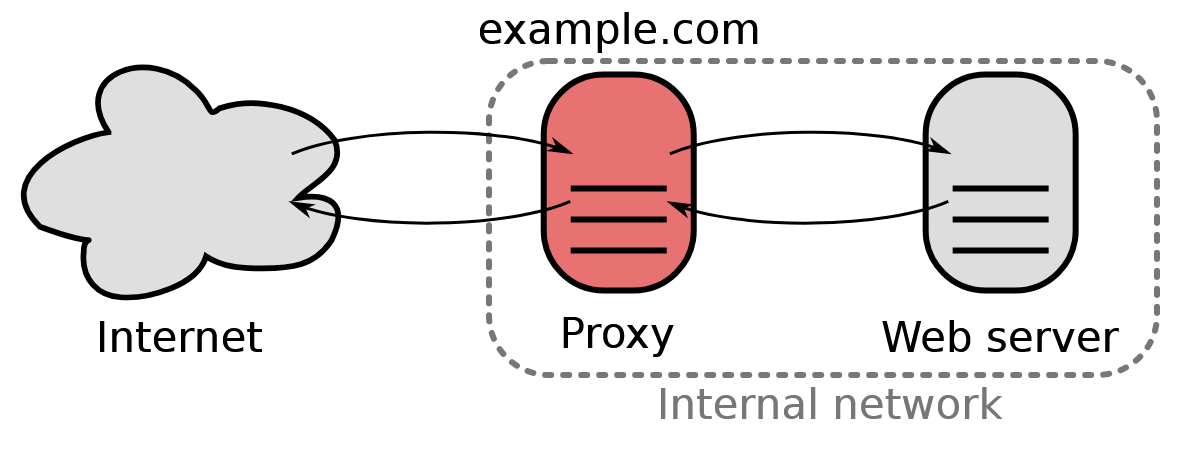
\includegraphics[width=0.7\textwidth]{img/proxy.png} \cite{proxy}
	\end{center}
\end{frame}

\begin{frame}[fragile]{SOCKS Proxy}
	Use a server as a \emph{SOCKS} proxy:
	\begin{lstlisting}
$ ssh -D 1080 -N server.example.org
	\end{lstlisting}
	\texttt{-N} can be used to not start a shell on the server.

	Use localhost with port 1080 in the proxy settings of your browser.
\end{frame}

\section{Port Forwarding}
\begin{frame}
	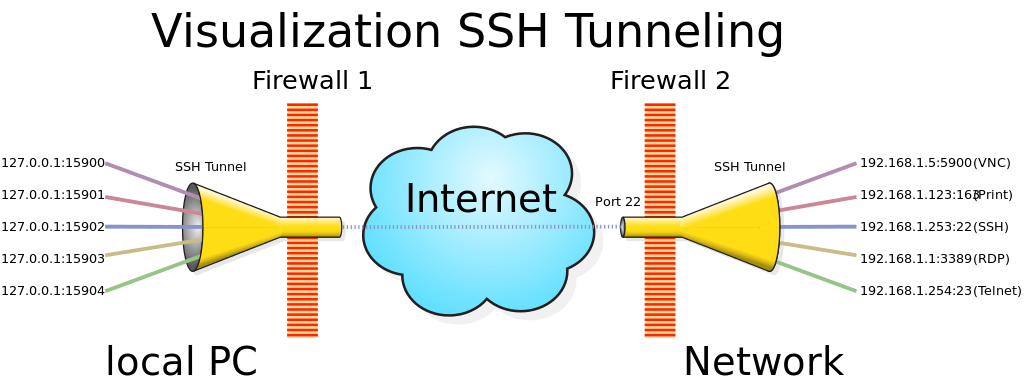
\includegraphics[width=\textwidth]{img/tunnel.png} \cite{tunnel}
\end{frame}

\begin{frame}[fragile]{Local Portforwarding}
	\textbf{Connect to a remote website which is blocked by a firewall:}
	\begin{lstlisting}
$ ssh -L 8080:localhost:80 server.example.org
$ ssh -L 8080:server.example.org:80 firewall.example.org
	\end{lstlisting}
\end{frame}

\begin{frame}[fragile]{Remote Portforwarding}
	\textbf{Make your local website accessible by programs on the server:}
	\begin{lstlisting}
$ ssh -R 80:localhost:8080 server.example.org
	\end{lstlisting}
\end{frame}

\section{Config File}
\begin{frame}[fragile]{Motivation}
	You are to lazy to type the awful long SSH commands?
	\begin{lstlisting}
$ ssh long_user_name@long.nasty.server.name -p 9999
	\end{lstlisting}
\end{frame}

\begin{frame}[fragile]{Config File}
	Configure an alias for your connection in the \textit{$\sim$/.ssh/config} file:
	\begin{lstlisting}
Host myserver
Hostname long.nasty.server.name
User long_user_name
Port 9999
ProxyJump firewall.example.com:22
LocalForward 8201 localhost:8200
	\end{lstlisting}

	Usage:
	\begin{lstlisting}
$ ssh myserver
	\end{lstlisting}
\end{frame}

\begin{frame}[fragile]{Applied Options}
	Show what options are applied on a connection:
	\begin{columns}
	\column{0.5\textwidth}
		\begin{lstlisting}
$ ssh -G switch-bu24.agdsn.network
user jakob
hostname switch-bu24.agdsn.network
port 22
[...]
proxyjump login.agdsn.tu-dresden.de
		\end{lstlisting}
	\column{0.5\textwidth}
		\begin{lstlisting}
Host switch-bu24.agdsn.network
User jakob
Host *
IdentitiesOnly yes
ControlMaster auto
ControlPersist 60s
Host login.agdsn.tu-dresden.de
ProxyCommand none
Hostname 141.76.119.134
Host *.agdsn *.agdsn.network
ProxyJump login.agdsn.tu-dresden.de
IdentityFile ~/.ssh/id_ed25519
		\end{lstlisting}
    \end{columns}
\end{frame}

\begin{frame}[fragile]{Reuse Connections}
	Multiple connections to a singe server is inefficient (e.g. in Robolab).
	\pause

	\textbf{How can you use a single connection for multiple sessions?}
	\begin{lstlisting}
Host *
ControlMaster auto
ControlPath ~/.ssh/sockets/%r@%h-%p
ControlPersist 600
	\end{lstlisting}
\end{frame}

\section{Copying Files}
\begin{frame}[fragile]{SCP}
	\textbf{How to copy a file from or to a server?}
	\pause

	\begin{lstlisting}
$ scp /file/on/my/machine remote_user@server:/destination
	\end{lstlisting}
	\pause

	And a directory?
	\begin{lstlisting}
$ scp -r /my/directory/ remote_user@server:/destination/
	\end{lstlisting}
	This also uses your SSH config.
\end{frame}

\begin{frame}[fragile]{SFTP}
	\begin{columns}
	\column{0.5\textwidth}<+->
		\begin{itemize}
			\item
				More elaborate operations\\
				(e.g. rename, deletion)
			\item Opens a session for multiple operations
			\item Has many graphical user interfaces
		\end{itemize}
	\column{0.5\textwidth}<+->
		\centering
		\emph{FileZilla}	 \cite{filezilla}
		\vspace{1ex}

		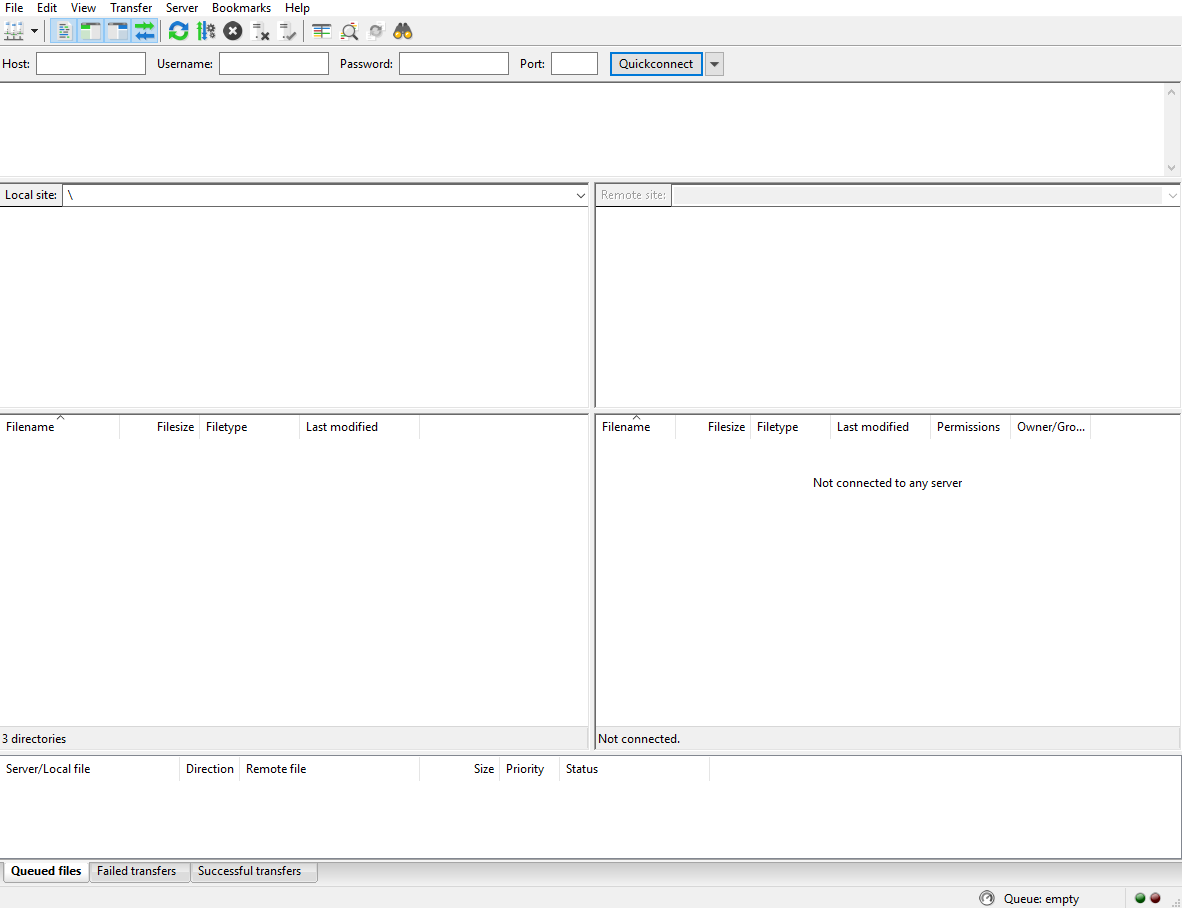
\includegraphics[width=\textwidth]{img/filezilla.png}
	\end{columns}
\end{frame}

\section{Windows}
\begin{frame}[fragile]{Help! I am using Windows.}
	\begin{columns}
	\column{0.5\textwidth}
		\begin{itemize}
			\item Install Linux
			\item Port of SSH in \textit{Git for Windows}
			\item Windows Subsystem for Linux
			\item Cross-platform SSH clients (e.g. \textit{PuTTY})
		\end{itemize}
	\column{0.5\textwidth}
		\centering
		\emph{PuTTY} \cite{putty}

		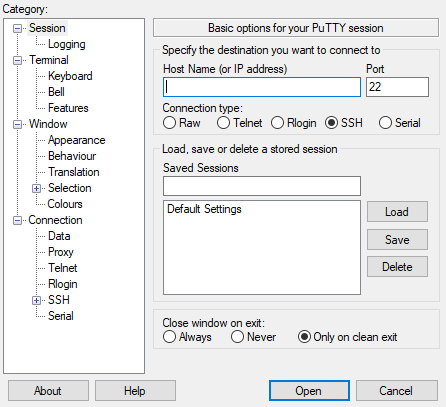
\includegraphics[height=0.65\paperheight]{img/putty.png}
	\end{columns}
\end{frame}

\section{References}
\begin{frame}[allowframebreaks]
	\printbibliography[heading=none]
\end{frame}

\end{document}
